\documentclass[12pt]{article}

\usepackage[margin=1in]{geometry}
\usepackage{listings}
\usepackage{xcolor}
\usepackage{graphicx}
\usepackage{float}

\lstset{
    basicstyle=\ttfamily\small,
    breaklines=true,
    frame=single,
    columns=fullflexible
}

\begin{document}

\begin{center}
    \Large \textbf{COSC 417 Programming Task 2 Writeup} \\[0.2in]
    \normalsize
    Jonathan Llovet, Matt Saxton, Amarachi King, Abdullah Radid \\[0.1in]
    \today
\end{center}

\section*{Program Description}

The goal of this program is to simulate a nondeterministic finite automaton, or NFA, on an input string. The program reads the NFA from a text file, then asks the user to enter an input string. After running the NFA on the input, the program prints \texttt{ACCEPT} if at least one possible computation path ends in an accepting state. If no possible path accepts the string, the program prints \texttt{REJECT}.


\section*{Data Structures Used}

The program represents the NFA using arrays/lists to store the states, accepting states, and transitions. Each transition stores three pieces of information: the old state, the symbol, and the new state. The symbol is either \texttt{0}, \texttt{1}, or \texttt{-1}, where \texttt{-1} represents an epsilon transition. A major part of the implementation is the use of Java \texttt{Set} structures. Sets are useful here because an NFA can have multiple active states at the same time, but the same state does not need to appear more than once. For example, after following several possible transitions, the program stores the current possible states in a \texttt{Set<Integer>}. This avoids duplicates automatically and makes it easier to compare groups of states.

Sets are also important for handling epsilon transitions. The epsilon closure is stored as a set because it represents all states reachable using zero or more epsilon moves. Since sets do not allow duplicates, they help prevent the program from repeatedly adding the same state during an epsilon cycle. This is what keeps the simulation from getting stuck forever when the NFA has cycles made only of epsilon transitions.

The input string is stored as a normal Java \texttt{String}. The program keeps track of both the current state and the current position in the input string. This is important because a computation path is not only based on what state the NFA is in, but also how much of the input has already been read.

\section*{How the Simulation Works}

The program explores possible NFA computations by checking every valid transition from the current state. If the transition matches the current input symbol, the program moves to the next state and advances the input position by one. If the transition is an epsilon transition, the program moves to the next state without advancing the input position.

This process continues until the program either finds an accepting path or runs out of possible paths. A string is accepted only if there is at least one path where the entire input string has been read and the final state is an accepting state.

\section*{Handling Epsilon Cycles}

One important part of the assignment is handling epsilon cycles. An epsilon cycle can cause the program to move between states forever without reading any new input. To avoid this problem, the program keeps track of configurations it has already visited.

A configuration is made up of the current state and the current position in the input string. If the program reaches the same state with the same input position again, it does not need to explore that path again. This prevents infinite loops while still allowing the program to check all useful possible paths.

\section*{Testing}

The program was tested using the NFA shown in the assignment. The required input strings were:

\begin{itemize}
    \item \texttt{0}
    \item \texttt{01}
    \item \texttt{110}
    \item \texttt{0100}
    \item \texttt{100}
\end{itemize}

For each input string, the program printed either \texttt{ACCEPT} or \texttt{REJECT} depending on whether the NFA accepted the string.

\section*{Program Code}

\begin{lstlisting}[language=Java]
import java.io.IOException;
import java.nio.file.Files;
import java.nio.file.Path;
import java.nio.file.Paths;
import java.util.*;

public class NFASimulator {

    private static final int EPSILON = -1;

    private int numStates;
    private Set<Integer> acceptingStates;
    private Map<String, Set<Integer>> transitions;

    public NFASimulator(String path) {
        acceptingStates = new HashSet<>();
        transitions = new HashMap<>();
        if (path != null && !path.isEmpty()) {
            try {
                buildNFAFromFile(path);
            } catch (Exception e) {
                System.err.println("Error building NFA from file, falling back to empty NFA");
            }
        }
    }

    public void addAcceptingState(int state) {
        if (state < 1 || state > 20)
            throw new IllegalArgumentException("Accepting state out of range: " + state);
        acceptingStates.add(state);
    }

    public void addTransition(int from, int symbol, int to) {
        if (from < 1 || from > 20 || to < 1 || to > 20)
            throw new IllegalArgumentException("State out of range in transition: " + from + " " + symbol + " " + to);
        if (symbol != 0 && symbol != 1 && symbol != EPSILON)
            throw new IllegalArgumentException("Symbol must be 0, 1, or -1, got: " + symbol);
        String key = from + "," + symbol;
        if (!transitions.containsKey(key)) {
            transitions.put(key, new HashSet<>());
        }
        transitions.get(key).add(to);
    }

    private List<String> readNFASpecFromFile(String path) {
        Path p = Paths.get(path);
        try {
            List<String> lines = Files.readAllLines(p);
            System.out.println("GOT LINES");
            return lines;
        } catch (IOException | SecurityException e) {
            System.err.println(e.getMessage());
            return null;
        }
    }

    private void buildNFAFromFile(String path) throws IOException, NumberFormatException {
        List<String> lines = readNFASpecFromFile(path);
        if (lines == null) {
            throw new IOException("Unable to read NFA definition from file at " + path);
        }

        // line 0: number of states
        try {
            numStates = Integer.parseInt(lines.get(0).trim());
        } catch (NumberFormatException e) {
            throw new NumberFormatException("Unable to parse number of states: " + lines.get(0));
        }

        // line 1: accepting states
        String[] accepting = lines.get(1).split(" ");
        for (String state : accepting) {
            try {
                int s = Integer.parseInt(state.trim());
                addAcceptingState(s);
            } catch (NumberFormatException e) {
                throw new NumberFormatException("Unable to parse accepting state: " + state);
            }
        }

        // lines 2+: transitions
        for (String transition : lines.subList(2, lines.size())) {
            if (transition.trim().isEmpty()) continue;
            try {
                String[] parts = transition.split("\\s+");
                int from   = Integer.parseInt(parts[0]);
                int symbol = Integer.parseInt(parts[1]);
                int to     = Integer.parseInt(parts[2]);
                addTransition(from, symbol, to);
            } catch (NumberFormatException e) {
                throw new NumberFormatException("Unable to parse transition: " + transition);
            }
        }
    }

    public String simulate(String w) {
        for (char c : w.toCharArray()) {
            if (c != '0' && c != '1')
                throw new IllegalArgumentException(
                    "Input must only contain strings of 0 or 1, got '" + c + "'");
        }

        Set<Integer> currentStates = new HashSet<>();
        currentStates.add(1);
        currentStates = epsilonClosure(currentStates);

        System.out.println("\nSimulating NFA...");
        System.out.println("Starting epsilon-closure({1}) = " + currentStates);

        for (char c : w.toCharArray()) {
            int symbol = c - '0';

            Set<Integer> moved = move(currentStates, symbol);
            Set<Integer> nextStates = epsilonClosure(moved);

            System.out.println("d(" + currentStates + ", " + c + ") = " + moved + ", epsilon-closure = " + nextStates);

            currentStates = nextStates;

            if (currentStates.isEmpty()) {
                System.out.println("No active states, NFA will reject");
                break;
            }
        }

        System.out.println("Final states: " + currentStates);

        Set<Integer> finalAccepting = new HashSet<>(currentStates);
        finalAccepting.retainAll(acceptingStates);
        return !finalAccepting.isEmpty() ? "ACCEPT" : "REJECT";
    }

    // computes all states reachable via zero or more epsilon transitions
    private Set<Integer> epsilonClosure(Set<Integer> states) {
        Set<Integer> closure = new HashSet<>(states);
        for (int state : states) {
            dfsEpsilon(state, closure);
        }
        return closure;
    }

    // recursive dfs following epsilon transitions, closure acts as visited set
    private void dfsEpsilon(int state, Set<Integer> closure) {
        String key = state + "," + EPSILON;
        Set<Integer> epsilonClosure = transitions.get(key);

        if (epsilonClosure == null) return;

        for (int next : epsilonClosure) {
            if (!closure.contains(next)) {
                closure.add(next);
                dfsEpsilon(next, closure);
            }
        }
    }

    // returns all states reachable by reading one symbol from the current set
    private Set<Integer> move(Set<Integer> states, int symbol) {
        Set<Integer> result = new HashSet<>();
        for (int state : states) {
            String key = state + "," + symbol;
            Set<Integer> reachable = transitions.get(key);
            if (reachable != null) {
                result.addAll(reachable);
            }
        }
        return result;
    }

    public static void main(String[] args) {
        String path = args.length > 0 ? args[0] : "nfa.txt";
        NFASimulator nfa = new NFASimulator(path);

        try (Scanner scan = new Scanner(System.in)) {
            while (true) {
                System.out.print("\nEnter input string w. (Enter 'quit' to exit)\n");
                String w = scan.nextLine().trim();

                if (w.equalsIgnoreCase("quit")) {
                    System.out.println("Exiting simulation");
                    break;
                }

                try {
                    String result = nfa.simulate(w);
                    System.out.println(result);
                } catch (IllegalArgumentException e) {
                    System.out.println("ERROR: " + e.getMessage());
                }
            }
        }
    }
}\end{lstlisting}

\section*{NFA Input File}

\begin{lstlisting}
3
1
1 1 2
2 0 2
2 0 3
2 1 3
3 0 1
3 -1 1
1 -1 3\end{lstlisting}

\section*{Program Output}

\begin{figure}[H]
    \centering
    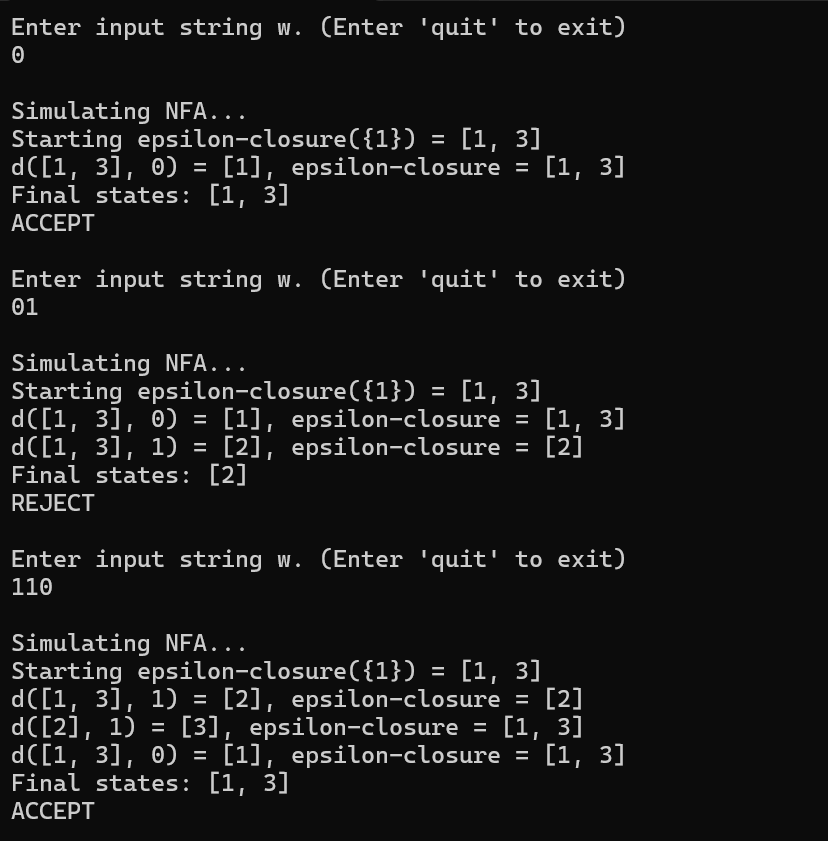
\includegraphics[width=0.9\textwidth]{output1.png}
    \caption{First program output screenshot}
\end{figure}

\begin{figure}[H]
    \centering
    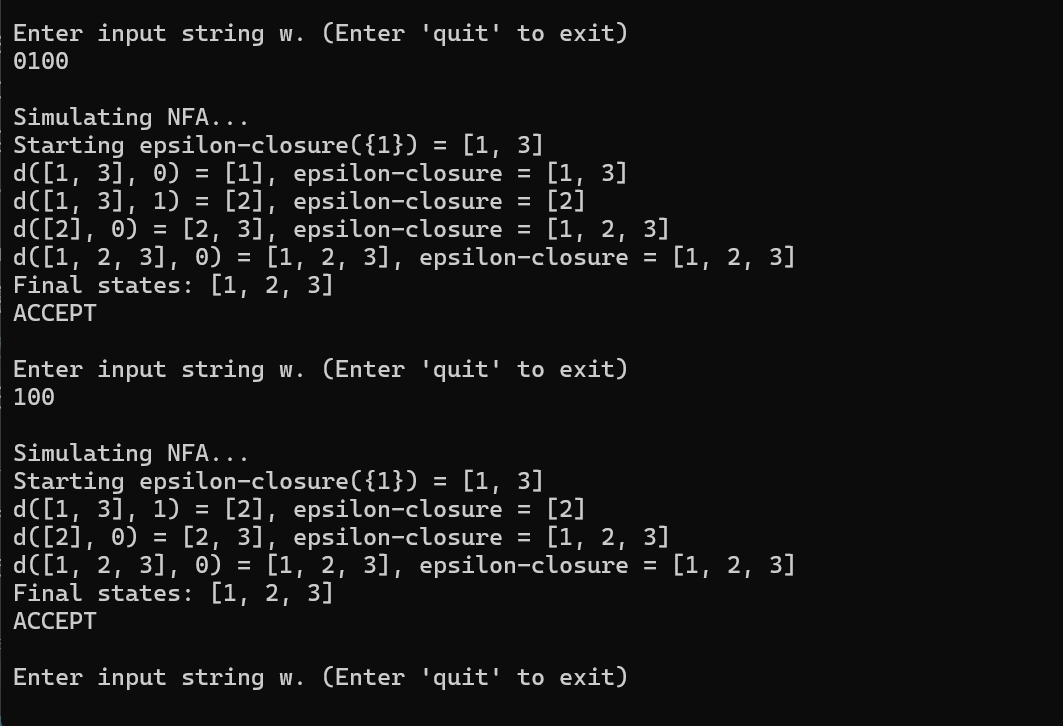
\includegraphics[width=0.9\textwidth]{output2.png}
    \caption{Second program output screenshot}
\end{figure}


\end{document}